\documentclass[aspectratio=169,11pt,svgnames]{beamer}

\usepackage[czech]{babel}
\usepackage[czech=quotes]{csquotes}
\usepackage{graphicx}
\usepackage{enumitem}
\usepackage{amsmath}
\usepackage{mathtools}
\usepackage{float}
\usepackage{tikz}

% Flowchart stuff
\usetikzlibrary{shapes.geometric, arrows.meta, calc, positioning}
\tikzstyle{startstop} = [rectangle, rounded corners, minimum width=3cm, minimum
height=1cm,text centered, draw=black, fill=Red!30]
\tikzstyle{io} = [trapezium, trapezium left angle=70, trapezium right angle=110,
minimum width=3cm, minimum height=1cm, text centered, draw=black, fill=Blue!30]
\tikzstyle{process} = [rectangle, minimum width=3cm, minimum height=1cm, text
centered, draw=black, fill=Orange!30]
\tikzstyle{decision} = [diamond, aspect=2, minimum width=3cm, minimum height=.5cm, text
centered, draw=black, fill=Green!30]
\tikzstyle{connector} = [draw, -latex']

\usepackage{pgfopts}
\usepackage{xcolor}
\usepackage{tcolorbox}
\usepackage{booktabs}

\usetheme[
 titlestyle=style2,
 titleformat=smallcaps,
 sectionstyle=plain,
 slidestyle=cyber,
 headingcolor=theme,
 block=transparent
]{trigon}

\title{Počítače a data}
\subtitle{Data, informace, bit, byte \\ Číselné soustavy}
\date{\today}
\author{Adam Klepáč}
\institute[GEVO]{Gymnázium Evolution Jižní Město}
\biglogo[width=.2\textwidth]{logo}
\smalllogo[width=.1\textwidth]{logo}
\titlegraphic{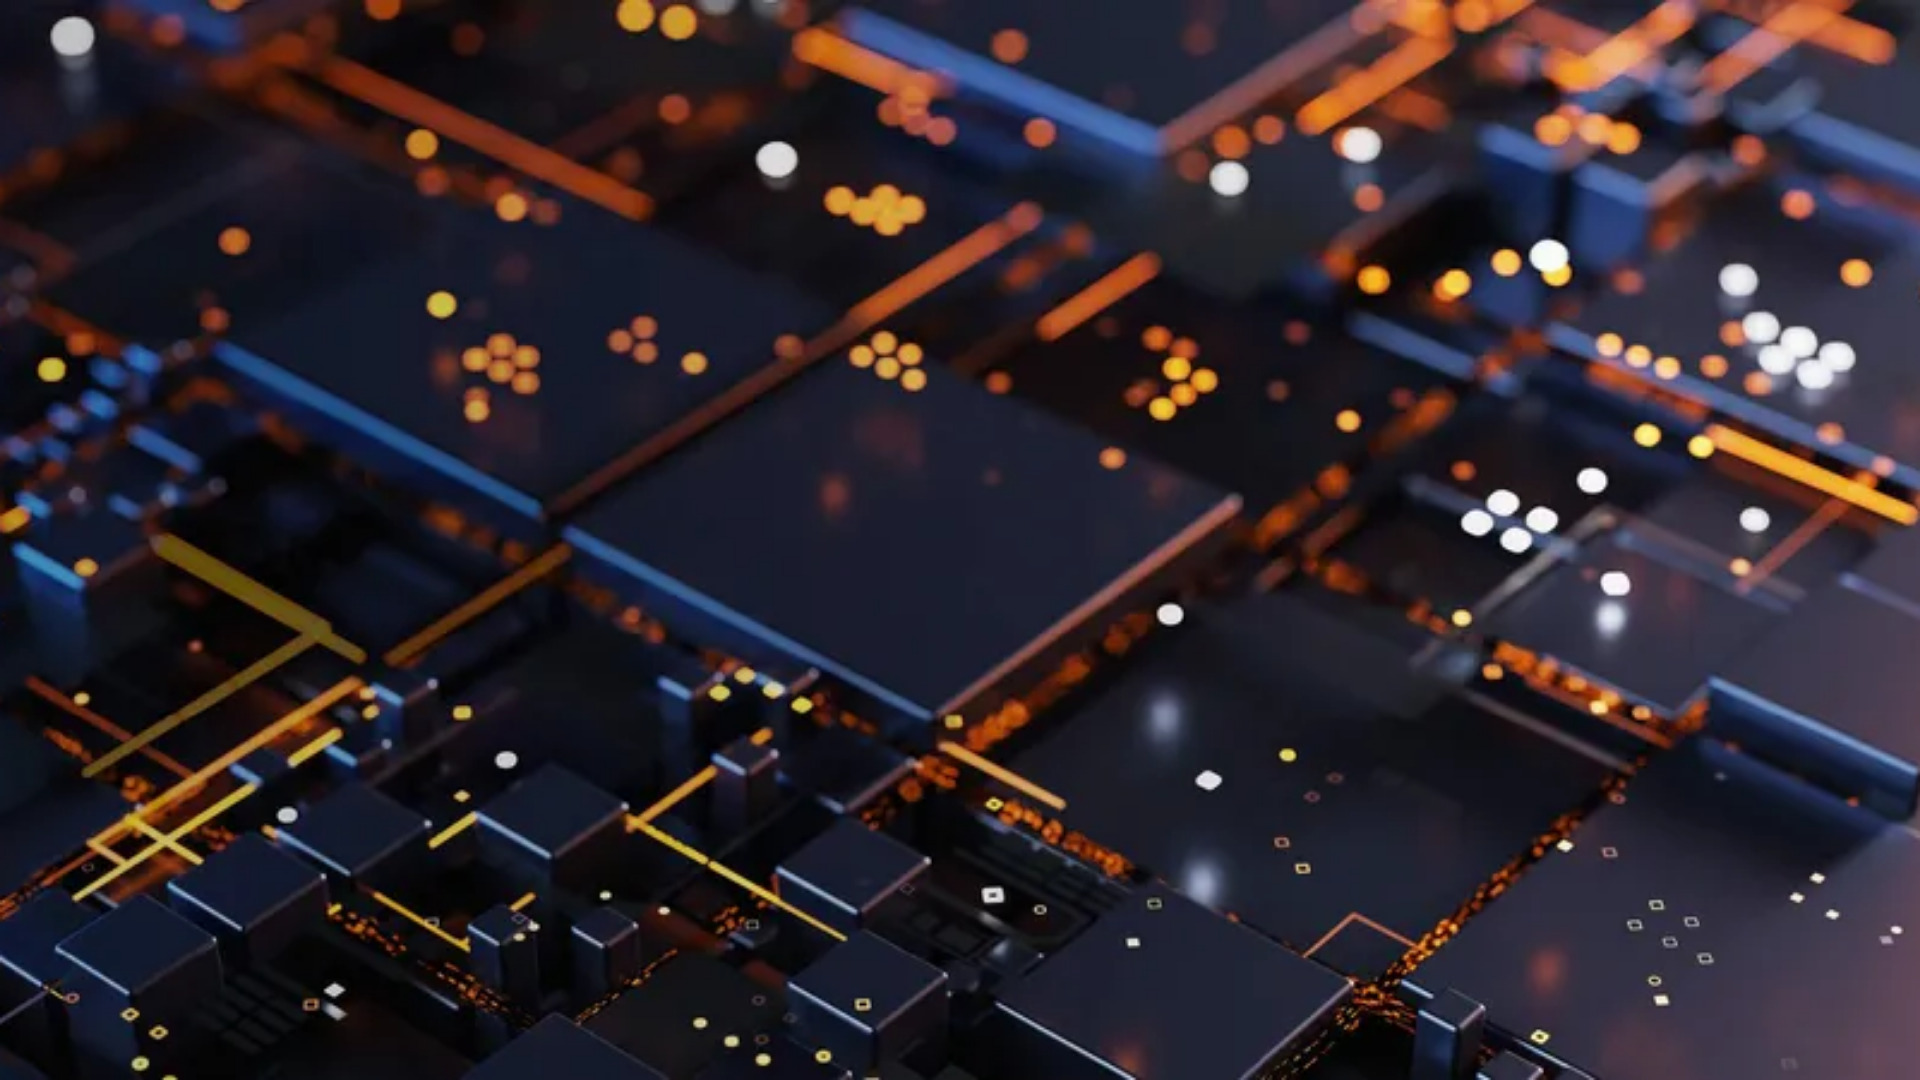
\includegraphics[height=\paperheight]{title.jpg}}

\def\subsectionname{}

% enumerate global settings
\setlist[enumerate,1]{label=\arabic*.}
\setlist[enumerate,2]{label=\alph*)}

% custom colors %
\definecolor{PCBlack}{HTML}{1B1B26}
\definecolor{PCBrown}{HTML}{642917}
\definecolor{PCGray}{HTML}{A6A7B5}
\definecolor{PCLavender}{HTML}{504456}
\definecolor{PCOrange}{HTML}{D16D1F}
\definecolor{PCBlue}{HTML}{2F4674}

\colorlet{tPrim}{PCBrown}
\colorlet{tSec}{PCLavender}
\colorlet{tAccent}{PCOrange}
\colorlet{tTheme}{PCBlue}
\colorlet{tTxt}{PCBlack}

\tcbset{
 boxsep=7pt,
 fonttitle=\sc,
 colframe=tGreyBg,
 colframe=tTheme,
 boxrule=1pt
}

\begin{document}
\titleframe

\begin{frame}
 \frametitle{Obsah}
 \tableofcontents
\end{frame}

\section{Data vs. Informace}

\begin{frame}
 \frametitle{Data}
 \begin{tcolorbox}[title=Datum]
  \alert{Datum} můžeme vnímat jako reprezentaci faktů, konceptů nebo instrukcí
  způsobem dostatečně formálním na to, aby mohlo být interpretováno nebo
  vykonáno člověkem či přístrojem.
 \end{tcolorbox}
\end{frame}

\begin{frame}
 \frametitle{Data -- Příklady}
 \begin{block}{Co můžeme nazvat datem}
  \begin{itemize}[label=\textbullet]
   \item<1-> \uv{Zítra bude pršet.} je datum -- fakt, který člověk umí interpretovat.
   \item<2-> \uv{Sečti $2$ a $5$.} je datum -- instrukce, kterou umí člověk, a v
    mnoha podobách i počítač, interpretovat.
   \item<3-> \uv{(255,0,0)} je většinou datum -- koncept, který umí počítač
    (prostřednictvím překladače programovacího jazyka) interpretovat jako
    červenou barvu.
  \end{itemize}
 \end{block}
\end{frame}

\begin{frame}
 \frametitle{Data -- Příklady}
 \begin{block}{Co datum spíš není}
  \begin{itemize}[label=\textbullet]
   \item<1-> \uv{1,kuře,juxtapozice,feromon} -- náhodná sada slov a symbolů bez
    kontextu nic nereprezentuje, přestože každý z nich má odděleně význam.
   \item<2-> zemětřesení (obecně jakákoli událost) -- údaj o tom, že se událost
    stala, datem \alert{je}, ta samotná událost \alert{není}.
   \item<3-> obecně předměty -- zase, to, že se s předmětem něco děje, datum
    \alert{je}, ten samotný předmět \alert{ne}.
  \end{itemize}
 \end{block}
\end{frame}

\begin{frame}
 \frametitle{Informace}
 \begin{tcolorbox}[title=Informace]
  Informace jsou \alert{data}, která jsou \emph{seřazena} nebo \emph{roztříděna}
  a mají hodnotu pro příjemce. Jsou to zpracovaná data, jimiž se řídí budoucí
  činy a rozhodnutí.
 \end{tcolorbox}
\end{frame}

\begin{frame}
 \frametitle{Informace -- Charakteristiky}
 Aby mohlo být datum pro příjemce užitečné (a tedy být \alert{informací}), musí
 být
 \begin{itemize}[label=\textbullet]
  \item<2-> \alert{včasné} -- poskytnuto v době, kdy je stále relevantní;
  \item<3-> \alert{přesné} -- neobsahující chyby a víceznačné formulace;
  \item<4-> \alert{úplné} -- žádná část důležitá pro interpretaci nesmí chybět.
 \end{itemize}
\end{frame}

\begin{frame}
 \frametitle{Informace -- Příklady}
 V jazyce občas říkáme \uv{zbytečná informace}. Bacha na to! Informace \alert{z
 definice} není pro příjemce zbytečná. \uv{Zbytečná informace} je tudíž prostě
 \alert{datum}.
 \pause
 \begin{block}{Kdy datum je a kdy není informací?}
  \begin{itemize}[label=\textbullet]
   \item<2-> V moment, kdy nakupuji, je datum ceny produktu informací.
    \begin{itemize}[label=\textminus]
    \item<3-> Je \alert{včasné}? \checkmark \; Nakupuji \emph{teď}.
    \item<4-> Je \alert{přesné}? \checkmark \; Nemůže se stát, že bych produkt
     koupil za jinou cenu.
    \item<5-> Je \alert{úplné}? \checkmark \; Ano, číslo vyjadřuje absolutní
     hodnotu.
   \end{itemize}
  \end{itemize}
 \end{block}
\end{frame}

\begin{frame}
 \frametitle{Informace -- Příklady}
 \begin{block}{Kdy datum je a kdy není informací?}
  \begin{itemize}[label=\textbullet]
   \item<1-> Vzkaz \uv{Supluješ první hodinu v pondělí.} řečený v úterý odpoledne
    \emph{není} informací. Je sice \alert{přesný}, ale není ani \alert{včasný}
    ani \alert{úplný}.
   \item<2-> Příkaz \uv{Sečti nebo vyděl dvě čísla.} není informací. Je sice
    \alert{včasný}, ale ani \alert{přesný} ani \alert{úplný}.
  \end{itemize}
 \end{block}
\end{frame}

\begin{frame}
 \frametitle{Datum $ \to $ Informace (Data Processing/Zpracování dat)}
 V nejširším slova smyslu jsou počítače stroje, které \alert{data} převádějí na
 \alert{informace}.\\
 \pause
 Každý počítačový program je \alert{cyklus zpracování dat}.
 \pause
 \begin{figure}[H]
  \centering
  \begin{tikzpicture}
   \node[draw,rectangle,white,fill=PCBlue,minimum width=3cm,minimum
    height=2cm,align=center] (input) at (0,0) {vstup \\ (datum)};
   \node[draw,rectangle,white,fill=PCBlue,minimum width=3cm,minimum
    height=2cm,align=center] (processing) at (5,0) {zpracování};
   \node[draw,rectangle,white,fill=PCBlue,minimum width=3cm,minimum
    height=2cm,align=center] (output) at (10,0) {výstup \\ (informace)};
   \draw[-{Latex[scale=1]},thick] (input) -- (processing);
   \draw[-{Latex[scale=1]},thick] (processing) -- (output);
  \end{tikzpicture}
 \end{figure}
\end{frame}

\begin{frame}
 \frametitle{Datum $ \to $ Informace (Data Processing/Zpracování dat)}
 \begin{figure}[H]
  \centering
  \begin{tikzpicture}
   \node[draw,rectangle,white,fill=PCBlue,minimum width=3cm,minimum
    height=2cm,align=center] (input) at (0,0) {vstup \\ (datum)};
   \node[draw,rectangle,white,fill=PCBlue,minimum width=3cm,minimum
    height=2cm,align=center] (processing) at (5,0) {zpracování};
   \node[draw,rectangle,white,fill=PCBlue,minimum width=3cm,minimum
    height=2cm,align=center] (output) at (10,0) {výstup \\ (informace)};
   \draw[-{Latex[scale=1]},thick] (input) -- (processing);
   \draw[-{Latex[scale=1]},thick] (processing) -- (output);
  \end{tikzpicture}
 \end{figure}
 \pause
 \begin{itemize}[label=\textbullet]
  \item<2-> \alert{vstup} (input) -- data ve formě umožňující zpracování
  \item<3-> \alert{zpracování} (processing) -- data jsou transformována v data
   užitečnější
  \item<4-> \alert{výstup} (output) -- transformovaná jsou sesbírána a předána
   jako informace
 \end{itemize}
\end{frame}

\begin{frame}
 \frametitle{Cyklus zpracování dat -- Příklady}
 \begin{block}{Náš mozek zpracovává data neustále.}
  \begin{itemize}[label=\textbullet]
   \item<1-> Smysly -- paprsky světla nebo vibrace ve vzduchu jsou \alert{data},
    nejsou nám nijak užitečná. Smysly jsou způsob, jak náš mozek dostává
    \alert{vstup}. \alert{Výstupem} je jakýsi model našeho okolí.
   \item<2-> Logika -- vzkaz \uv{Zastávka na znamení.} je \alert{datum}, není v
    užitečné formě. Je \alert{vstupem}, který vyhodnotíme (\alert{zpracujeme}) a
    vyrobíme z něj \alert{výstup} -- informaci, že musíme zmáčknout tlačítko,
    abychom směli vystoupit.
  \end{itemize}
 \end{block}
\end{frame}

\begin{frame}
 \frametitle{Cyklus zpracování dat -- Příklady}
 \begin{block}{Teď něco s počítačem...}
  \begin{itemize}[label=\textbullet]
   \item<1-> Sečti čísla $2$ a $3$.
   \begin{itemize}[label=\textminus]
    \item<2-> \alert{Vstupem} jsou čísla $2$ a $3$.
    \item<3-> \alert{Zpracování} spočívá v provedení operace součtu.
    \item<4-> \alert{Výstupem} je číslo $5$.
   \end{itemize}
  \item<5-> Otevření aplikace.
  \begin{itemize}[label=\textminus]
   \item<6-> \alert{Vstupem} jsou dvě kliknutí na ikonku.
   \item<7-> \alert{Zpracování} spočívá v otevření aplikace s odpovídající ikonkou.
   \item<8-> \alert{Výstupem} je okno s otevřenou aplikací.
  \end{itemize}
  \end{itemize}
 \end{block}
\end{frame}

\section{Bit a byte}

\begin{frame}
 \frametitle{Co je bit}
 \begin{tcolorbox}[title=Bit]
  \alert{Bit} (\textbf{bi}nary digi\textbf{t}) je nejmenší datová jednotka,
  která může být uložena v paměti počítače.
 \end{tcolorbox}
\end{frame}

\begin{frame}
 \frametitle{Jednotky počítačové paměti}
 \begin{table}[H]
  \centering
  \begin{tabular}{c|p{.7\textwidth}}
   \textbf{Název} & \textbf{Popis} \\
   \toprule
   bit & Logická $0$ (\uv{ne}) nebo $1$ (\uv{ano}) představující stav komponenty
   elektrického obvodu.\\
   \midrule
   nibble & Skupina $4$ bitů. \alert{Nepoužívá se}.\\
   \midrule
   byte (B) & Skupina $8$ bitů.\\
   \midrule
   slovo (word) & Skupina fixního počtu bitů. Různá procesor od procesoru
   (obvykle mezi $8$ a $96$ bity).
  \end{tabular}
 \end{table}
\end{frame}

\begin{frame}
 \frametitle{Jednotky počítačové paměti}
 \begin{table}[H]
  \centering
  \begin{tabular}{c|c}
   \textbf{Název} & \textbf{Popis} \\
   \toprule
   \textbf{kilo}byte (KB) & 1024 bytů.\\
   \midrule
   \textbf{mega}byte (MB) & 1024 KB = 1048576 B.\\
   \midrule
   \textbf{giga}byte (GB) & 1024 MB = 1073741824 B.\\
   \midrule
   \textbf{tera}byte (TB) & 1024 GB = 1099511628000 B.
  \end{tabular}
 \end{table}
\end{frame}

\section{Číselné soustavy}

\begin{frame}
 \frametitle{Hodnota číslice}
 Počítače umějí interpretovat pouze čísla. Hodnota každé číslice v čísle je dána
 \begin{itemize}[label=\textbullet]
  \item<2-> tou číslicí,
  \item<3-> pozicí této číslice v čísle,
  \item<4-> základem číselné soustavy (počtu číslic, které jsou v dané soustavě
   k dispozici).
 \end{itemize}
\end{frame}

\begin{frame}
 \frametitle{Hodnota číslice -- příklad}
 \begin{figure}[H]
  \centering
  \begin{tikzpicture}
   \node[draw,rectangle,PCLavender,inner sep=6pt] at (0,0) {\LARGE $5$};
   \node[draw,rectangle,PCLavender,inner sep=6pt] at (1,0) {\LARGE $1$};
   \node[draw,thick,rectangle,PCOrange,inner sep=6pt] (digit) at (2,0) {\LARGE
    $2$};
   \node[draw,rectangle,PCLavender,inner sep=6pt] at (3,0) {\LARGE $6$};
   \node[draw,rectangle,PCLavender,inner sep=6pt] at (4,0) {\LARGE $7$};

   \node[align=left,draw,rectangle,inner sep=6pt,below=1cm of digit] (desc) {
     číslice: \alert{2},\\
     pozice: \alert{stovky},\\
     soustava: \alert{10}
    };
   \draw[-Latex,PCOrange] (digit) -- (desc);
  \end{tikzpicture}
 \end{figure}
\end{frame}

\begin{frame}
 \frametitle{Desítková soustava}
 Desítkovou soustavu používáme nejčastěji (protože máme deset prstů).\\
 \pause
 Používá číslice od $0$ do $9$.\\
 \pause
 Každé číslo v desítkové soustavě lze rozložit na součet násobků mocnin čísla
 $10$.
 \pause
 Například:
 \begin{align*}
  4321 &= (4 \cdot 1000) + (3 \cdot 100) + (2 \cdot 10) + (1 \cdot 1)\\
       &= (4 \cdot 10^{3}) + (3 \cdot 10^2) + (2 \cdot 10^{1}) + (1 \cdot
       10^{0}).
 \end{align*}
\end{frame}

\begin{frame}
 \frametitle{Další soustavy běžné v informatice}
 \begin{table}[H]
  \centering
  \begin{tabular}{c|l}
   \textbf{Název} & \textbf{Popis} \\
   \toprule
   dvojková (binární) & Základ \alert{2}. Číslice $0$ a $1$.\\
   \midrule
   osmičková (oktální) & Základ \alert{8}. Číslice od $0$ do $7$.\\
   \midrule
   šestnáctková (hexadecimální) & Základ \alert{16}. Číslice od $0$ do $9$ a
   písmena od A do F. \\
  \end{tabular}
 \end{table}
\end{frame}

\begin{frame}
 \frametitle{Příklad -- sčítání v osmičkové soustavě}
 \begin{figure}[H]
  \centering
  \begin{tikzpicture}
   \node[draw,rectangle,PCLavender,inner sep=6pt] at (0,1.5) {\LARGE $5$};
   \node[draw,rectangle,PCLavender,inner sep=6pt] at (1,1.5) {\LARGE $1$};
   \node[draw,rectangle,PCLavender,inner sep=6pt] at (2,1.5) {\LARGE $2$};
   \node[draw,rectangle,PCLavender,inner sep=6pt] at (3,1.5) {\LARGE $6$};
   \node[draw,rectangle,PCLavender,inner sep=6pt] at (4,1.5) {\LARGE $7$};

   \node[draw,rectangle,PCLavender,inner sep=6pt] at (0,0) {\LARGE $1$};
   \node[draw,rectangle,PCLavender,inner sep=6pt] at (1,0) {\LARGE $2$};
   \node[draw,rectangle,PCLavender,inner sep=6pt] at (2,0) {\LARGE $1$};
   \node[draw,rectangle,PCLavender,inner sep=6pt] at (3,0) {\LARGE $4$};
   \node[draw,rectangle,PCLavender,inner sep=6pt] at (4,0) {\LARGE $6$};
   
   \pause
   \node[draw,rectangle,thick,PCOrange,inner sep=6pt] (d15) at (4,1.5) {\LARGE\bf $7$};
   \node[draw,rectangle,thick,PCOrange,inner sep=6pt] (d25) at (4,0) {\LARGE\bf $6$};
   \node[PCOrange] at (4,0.75) {\LARGE\bf $+$};

   \node[draw,rectangle,thick,PCLavender,inner sep=6pt] (d35) at (4,-1.5) {\LARGE\bf $5$};
   \draw[-Latex,PCOrange] (d25) -- (d35);
   
   \pause
   \node[draw,rectangle,thick,PCOrange,inner sep=6pt] (d14) at (3,1.5) {\LARGE\bf $6$};
   \node[draw,rectangle,thick,PCOrange,inner sep=6pt] (d24) at (3,0) {\LARGE\bf $4$};
   \node[PCOrange] at (3,0.75) {\LARGE\bf $+$};                 
                                                                
   \node[draw,rectangle,thick,PCLavender,inner sep=6pt] (d34) at (3,-1.5) {\LARGE\bf $3$};
   \draw[-Latex,PCOrange] (d24) -- (d34);

   \pause
   \node[draw,rectangle,thick,PCOrange,inner sep=6pt] (d13) at (2,1.5) {\LARGE\bf $2$};
   \node[draw,rectangle,thick,PCOrange,inner sep=6pt] (d23) at (2,0) {\LARGE\bf $1$};
   \node[PCOrange] at (2,0.75) {\LARGE\bf $+$};                 
                                                                
   \node[draw,rectangle,thick,PCLavender,inner sep=6pt] (d33) at (2,-1.5) {\LARGE\bf $4$};
   \draw[-Latex,PCOrange] (d23) -- (d33);

   \pause
   \node[draw,rectangle,thick,PCOrange,inner sep=6pt] (d12) at (1,1.5) {\LARGE\bf $1$};
   \node[draw,rectangle,thick,PCOrange,inner sep=6pt] (d22) at (1,0) {\LARGE\bf $2$};
   \node[PCOrange] at (1,0.75) {\LARGE\bf $+$};                 
                                                                
   \node[draw,rectangle,thick,PCLavender,inner sep=6pt] (d32) at (1,-1.5) {\LARGE\bf $3$};
   \draw[-Latex,PCOrange] (d22) -- (d32);

   \pause
   \node[draw,rectangle,thick,PCOrange,inner sep=6pt] (d11) at (0,1.5) {\LARGE\bf $5$};
   \node[draw,rectangle,thick,PCOrange,inner sep=6pt] (d21) at (0,0) {\LARGE\bf $1$};
   \node[PCOrange] at (0,0.75) {\LARGE\bf $+$};                 
                                                                
   \node[draw,rectangle,thick,PCLavender,inner sep=6pt] (d31) at (0,-1.5) {\LARGE\bf $6$};
   \draw[-Latex,PCOrange] (d21) -- (d31);
  \end{tikzpicture}
 \end{figure}
\end{frame}

\begin{frame}
 \frametitle{Příklad -- sčítání v šestnáctkové soustavě}
 \begin{figure}[H]
  \centering
  \begin{tikzpicture}
   \node[draw,rectangle,PCLavender,inner sep=6pt] at (0,1.5) {\LARGE B};
   \node[draw,rectangle,PCLavender,inner sep=6pt] at (1,1.5) {\LARGE $8$};
   \node[draw,rectangle,PCLavender,inner sep=6pt] at (2,1.5) {\LARGE F};
   \node[draw,rectangle,PCLavender,inner sep=6pt] at (3,1.5) {\LARGE A};
   \node[draw,rectangle,PCLavender,inner sep=6pt] at (4,1.5) {\LARGE $5$};
   \node[draw,rectangle,PCLavender,inner sep=6pt] at (5,1.5) {\LARGE D};
   \node[draw,rectangle,PCLavender,inner sep=6pt] at (6,1.5) {\LARGE F};
   \node[draw,rectangle,PCLavender,inner sep=6pt] at (7,1.5) {\LARGE $8$};

   \node[draw,rectangle,PCLavender,inner sep=6pt] at (0,0) {\LARGE $2$};
   \node[draw,rectangle,PCLavender,inner sep=6pt] at (1,0) {\LARGE $5$};
   \node[draw,rectangle,PCLavender,inner sep=6pt] at (2,0) {\LARGE B};
   \node[draw,rectangle,PCLavender,inner sep=6pt] at (3,0) {\LARGE $3$};
   \node[draw,rectangle,PCLavender,inner sep=6pt] at (4,0) {\LARGE $6$};
   \node[draw,rectangle,PCLavender,inner sep=6pt] at (5,0) {\LARGE 0};
   \node[draw,rectangle,PCLavender,inner sep=6pt] at (6,0) {\LARGE F};
   \node[draw,rectangle,PCLavender,inner sep=6pt] at (7,0) {\LARGE $7$};
   
   \pause
   \node[draw,rectangle,thick,PCOrange,inner sep=6pt] (d18) at (7,1.5) {\LARGE\bf $8$};
   \node[draw,rectangle,thick,PCOrange,inner sep=6pt] (d28) at (7,0) {\LARGE\bf $7$};
   \node[PCOrange] at (7,0.75) {\LARGE\bf $+$};

   \node[draw,rectangle,thick,PCLavender,inner sep=6pt] (d38) at (7,-1.5)
    {\LARGE F};
   \draw[-Latex,PCOrange] (d28) -- (d38);

   \pause
   \node[draw,rectangle,thick,PCOrange,inner sep=6pt] (d17) at (6,1.5) {\LARGE F};
   \node[draw,rectangle,thick,PCOrange,inner sep=6pt] (d27) at (6,0) {\LARGE F};
   \node[PCOrange] at (6,0.75) {\LARGE\bf $+$};

   \node[draw,rectangle,thick,PCLavender,inner sep=6pt] (d37) at (6,-1.5)
    {\LARGE E};
   \draw[-Latex,PCOrange] (d27) -- (d37);

   \pause
   \node[draw,rectangle,thick,PCOrange,inner sep=6pt] (d16) at (5,1.5) {\LARGE D};
   \node[draw,rectangle,thick,PCOrange,inner sep=6pt] (d26) at (5,0) {\LARGE 0};
   \node[PCOrange] at (5,0.75) {\LARGE\bf $+$};

   \node[draw,rectangle,thick,PCLavender,inner sep=6pt] (d36) at (5,-1.5)
    {\LARGE E};
   \draw[-Latex,PCOrange] (d26) -- (d36);

   \pause
   \node[draw,rectangle,thick,PCOrange,inner sep=6pt] (d15) at (4,1.5)
    {\LARGE 5};
   \node[draw,rectangle,thick,PCOrange,inner sep=6pt] (d25) at (4,0) {\LARGE 6};
   \node[PCOrange] at (4,0.75) {\LARGE\bf $+$};

   \node[draw,rectangle,thick,PCLavender,inner sep=6pt] (d35) at (4,-1.5)
    {\LARGE B};
   \draw[-Latex,PCOrange] (d25) -- (d35);
   
   \pause
   \node[draw,rectangle,thick,PCOrange,inner sep=6pt] (d14) at (3,1.5)
    {\LARGE A};
   \node[draw,rectangle,thick,PCOrange,inner sep=6pt] (d24) at (3,0) {\LARGE $3$};
   \node[PCOrange] at (3,0.75) {\LARGE\bf $+$};                 
                                                                
   \node[draw,rectangle,thick,PCLavender,inner sep=6pt] (d34) at (3,-1.5)
    {\LARGE D};
   \draw[-Latex,PCOrange] (d24) -- (d34);

   \pause
   \node[draw,rectangle,thick,PCOrange,inner sep=6pt] (d13) at (2,1.5)
    {\LARGE F};
   \node[draw,rectangle,thick,PCOrange,inner sep=6pt] (d23) at (2,0) {\LARGE B};
   \node[PCOrange] at (2,0.75) {\LARGE\bf $+$};                 
                                                                
   \node[draw,rectangle,thick,PCLavender,inner sep=6pt] (d33) at (2,-1.5)
    {\LARGE A};
   \draw[-Latex,PCOrange] (d23) -- (d33);

   \pause
   \node[draw,rectangle,thick,PCOrange,inner sep=6pt] (d12) at (1,1.5)
    {\LARGE 8};
   \node[draw,rectangle,thick,PCOrange,inner sep=6pt] (d22) at (1,0) {\LARGE 5};
   \node[PCOrange] at (1,0.75) {\LARGE\bf $+$};                 
                                                                
   \node[draw,rectangle,thick,PCLavender,inner sep=6pt] (d32) at (1,-1.5)
    {\LARGE E};
   \draw[-Latex,PCOrange] (d22) -- (d32);

   \pause
   \node[draw,rectangle,thick,PCOrange,inner sep=6pt] (d11) at (0,1.5)
    {\LARGE B};
   \node[draw,rectangle,thick,PCOrange,inner sep=6pt] (d21) at (0,0) {\LARGE 2};
   \node[PCOrange] at (0,0.75) {\LARGE\bf $+$};                 
                                                                
   \node[draw,rectangle,thick,PCLavender,inner sep=6pt] (d31) at (0,-1.5)
    {\LARGE D};
   \draw[-Latex,PCOrange] (d21) -- (d31);
  \end{tikzpicture}
 \end{figure}
\end{frame}

\begin{frame}
 \frametitle{Převod cokoliv $ \to $ desítková}
 Když je třeba, píšeme u čísel soustavu v dolním indexu.\\
 \pause
 Například $4056_{10}$ je číslo $4056$ v desítkové soustavě, $A4578FB_{16}$ je
 číslo $A4578FB$ v~šestnáctkové soustavě a $1000101_2$ je číslo $1000101$
 dvojkové soustavě.\\
 \pause
 \begin{itemize}[label=\textbullet]
  \item Číslo se v každé soustavě \alert{rozkládá na součet násobků mocnin} 10.
  \item Abychom převedli číslo z libovolné soustavy do desítkové, stačí tedy
   číslo $10$ převést do desítkové soustavy a pak násobky mocnin sečíst.
  \item To je snadné, protože $10$ je vždy základ soustavy.
 \end{itemize}
\end{frame}

\begin{frame}
 \frametitle{Převod cokoliv $ \to $ desítková -- příklad}
 Vezměme třeba číslo $10011101_2$. To se v dvojkové soustavě rozkládá jako
 \begin{align*}
  10011101_2 &= 1 \cdot 10_2^{7} + 0 \cdot 10_2^{6} + 0 \cdot 10_2^{5} + 1 \cdot
  10_2^{4} + 1 \cdot 10^{3}_2 + 1 \cdot 10_2^{2} + 0 \cdot 10^{1}_2 + 1 \cdot
  10_2^{0}\\
             &= 10_2^{7} + 10_2^{4} + 10_2^{3} + 10_2^2 + 10_2^{0}.
 \end{align*}
 \pause
 Ale, $10_2 = 2_{10}$. Čili, v desítkové soustavě je to číslo
 \[
  2^{7} + 2^{4} + 2^{3} + 2^2 + 2^{0} = 157.
 \]
 \pause
 Takže,
 \[
  10011101_{2} = 157_{10}.
 \]
\end{frame}

\begin{frame}
 \frametitle{Převod desítková $ \to $ cokoliv}
 \begin{itemize}[label=\textbullet]
  \item<1-> Opačný postup nebude efektivní, protože neumíme rychle počítat v jiných
   soustavách.
  \item<2-> Místo toho využijeme tzv. \emph{Hornerova schématu}.
  \item<3-> To je způsob, jak rozdělit dané číslo na součet násobků mocnin
   libovolného jiného čísla \uv{opakovaným vytýkáním}.
  \item<4-> Při převodu z desítkové soustavy do soustavy se základem $a$ tedy
   stačí pořád dokola z tohoto čísla vytýkat $a$, dokud se nedostanu na $1$.
 \end{itemize}
\end{frame}

\begin{frame}
 \frametitle{Převod desítková $ \to $ cokoliv -- příklad}
 Převedeme číslo $49_{10}$ do dvojkové soustavy, tím že z něj budeme opakovaně
 vytýkat dvojku.\\
 \pause
 \vspace*{-2em}
 \begin{align*}
  49 &= 2 \cdot (24) + 1\\
     &= 2 \cdot (2 \cdot (12)) + 1\\
     &= 2 \cdot (2 \cdot (2 \cdot (6))) + 1\\
     &= 2 \cdot (2 \cdot (2 \cdot (2 \cdot (3)))) + 1\\
     &= 2 \cdot (2 \cdot (2 \cdot (2 \cdot (2 \cdot (1) + 1)))) + 1\\
     &= 2^{5} + 2^{4} + 2^{0}\\
     &= 10_2^{5} + 10_2^{4} + 10_2^{0}\\
     &= 1 \cdot 10_2^{5} + 1 \cdot 10_2^{4} + 0 \cdot 10_2^3 + 0 \cdot 10_2^2 +
     0 \cdot 10_2^{1} + 1 \cdot 10_2^{0} = 110001_2.
 \end{align*}
\end{frame}

\begin{frame}
 \frametitle{Převod desítková $ \to $ cokoliv -- příklad}
 Ten samý postup se přehledněji zapíše do tabulky.\\
 \pause
 Totiž, opakovaně vytýkat dvojku vlastně znamená opakovaně dělit číslo $2$ se
 zbytkem.
 \pause
 Pro číslo 49 vypadá tabulka následovně.
 \vspace*{-1em}
 \begin{table}[H]
  \centering
  \begin{tabular}{c|c}
   \textbf{Podíl} & \textbf{Zbytek}\\
   \toprule
   24 & 1\\
   12 & 0\\
   6 & 0\\
   3 & 0\\
   1 & 1 \\
   0 & 1
  \end{tabular}
 \end{table}
 \pause
 Když sloupec se zbytky přečteme zezdola nahoru, objevíme číslo $110001$, což je
 číslo $49$ ve dvojkové soustavě.
\end{frame}

\end{document}
